\documentclass[a4paper]{article}

\usepackage[T1]{fontenc}
\usepackage[utf8]{inputenc}
\usepackage{graphicx}
\usepackage{color}
\usepackage[intlimits]{amsmath}
\usepackage{amsfonts}
\usepackage{listings}
\usepackage{float}
\usepackage{setspace}
\usepackage[english]{babel}
\usepackage{fancyhdr}
\usepackage{booktabs}
\usepackage{multirow}
\usepackage{lastpage}
\usepackage[arrowmos]{circuitikz}
\usepackage[nottoc]{tocbibind}
\usepackage{url}
\usepackage[ugly]{units}
\usepackage[left=1.5cm,top=2cm,right=1.5cm,bottom=2.5cm]{geometry}
\usepackage[pdftex]{hyperref}
\usetikzlibrary{patterns,decorations.pathreplacing,automata,positioning,shapes,arrows}
\usepackage[T1]{fontenc}
%\usepackage{libertine}
\renewcommand*\oldstylenums[1]{{\fontfamily{fxlj}\selectfont #1}}
\setcounter{secnumdepth}{0}

\DeclareMathOperator{\ld}{ld}

\onehalfspacing
\setlength{\parindent}{0pt}

%\widowpenalty=1000
%\clubpenalty=1000

\tocsection

\author{Sophia Schillai}

\begin{document}
  \pdfinfo
  {/Creator (Sophia Schillai)
   /Producer (pdflatex)
   /Author (Sophia Schillai)
  }

\pagestyle{fancy}
\fancyhead{}
\fancyfoot{}
\renewcommand{\headrulewidth}{0pt}
\setlength{\parskip}{6pt}
\renewcommand{\headrulewidth}{.4pt}
\fancyhead[r]{Sophia Schillai, group 3}
\fancyhead[c]{Projektpraktikum IC-Entwurf}
\fancyhead[l]{Technische Universität München}
\fancyfoot[c]{Seite \thepage\ von \pageref{LastPage}}

\section{Uhrenbaustein}

\subsection{Overview}

\begin{figure}
  \begin{center}
    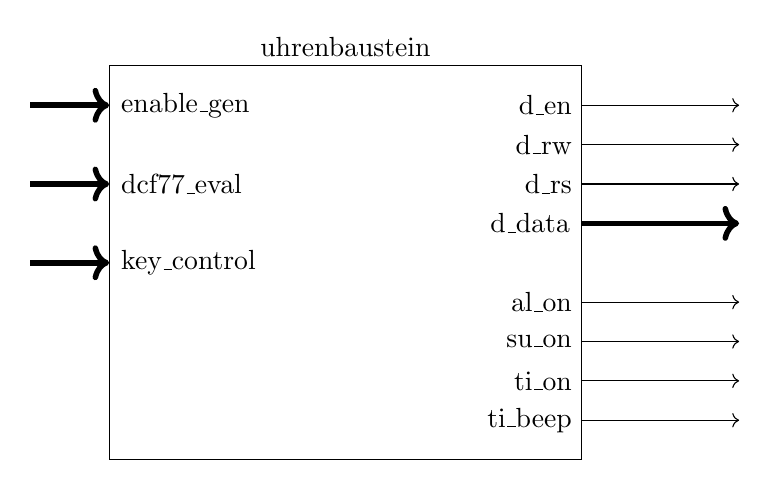
\begin{tikzpicture}
      \label{uhrenbaustein_overview}
%      \draw[help lines] (-2, -8) grid (7, 2);

      \node[above] at (3,0) {uhrenbaustein};

      \draw[line width=2pt,->] (-1, -0.5) -> (0, -0.5) node[right] { enable\_gen };
      \draw[line width=2pt,->] (-1, -1.5) -> (0, -1.5) node[right] { dcf77\_eval };
      \draw[line width=2pt,->] (-1, -2.5) -> (0, -2.5) node[right] { key\_control };

      \draw[->] (6,-0.5)node[left] {d\_en}   -- ++(2, 0);
      \draw[->] (6,-1)  node[left] {d\_rw}   -- ++(2, 0);
      \draw[->] (6,-1.5)node[left] {d\_rs}   -- ++(2, 0);
      \draw[line width=2pt,->] (6,-2) node[left] {d\_data} -- ++(2, 0);

      \draw[->] (6,-3)  node[left] {al\_on} -- ++(2, 0);
      \draw[->] (6,-3.5)node[left] {su\_on} -- ++(2, 0);
      \draw[->] (6,-4)  node[left] {ti\_on} -- ++(2, 0);
      \draw[->] (6,-4.5)node[left] {ti\_beep} -- ++(2, 0);

      \draw (0,0) rectangle (6, -5);
    \end{tikzpicture}
  \end{center}
  \caption{Block diagram of uhrenbaustein}
\end{figure}

In the top level-module Uhrenbaustein the inputs and outputs are supplied to all the submodules.
Besides general information like reset and the clock, this includes characters for the display, the current time and which modul currently reacts to the key input.


\subsection{Implementation}

The module Display Mux receives the display output as a three dimentsional array.
This three dimensional array is generated from the two dimensional outputs of the mudules in uhrenbaustein.
Display Mux then generates a two dimensional array for the display driver.
How the different signals for the display are handed through can be seen in% \ref{uhrenbaustein_char}.

The signals from the DCF77 transmitter are only handed to the Time Buffer module. All other modules receive their time signal (\texttt{ctime}) from this module.

The Mode FSM module receives all key inputs as well as the information if the alarm is currently ringing. 
From this information it decides, which module is currently active and reacts to the key input. 
It outputs a vector that is split into separate signals in Uhrenbaustein, \texttt{'1'} indicating that the module receiving this \texttt{keyboard\_focus} signal is active% (\ref{uhrenbaustein_time}).

The output \texttt{su\_on} is set to zero, since the stop watch module is not implemented.

\begin{figure}
  \begin{center}
    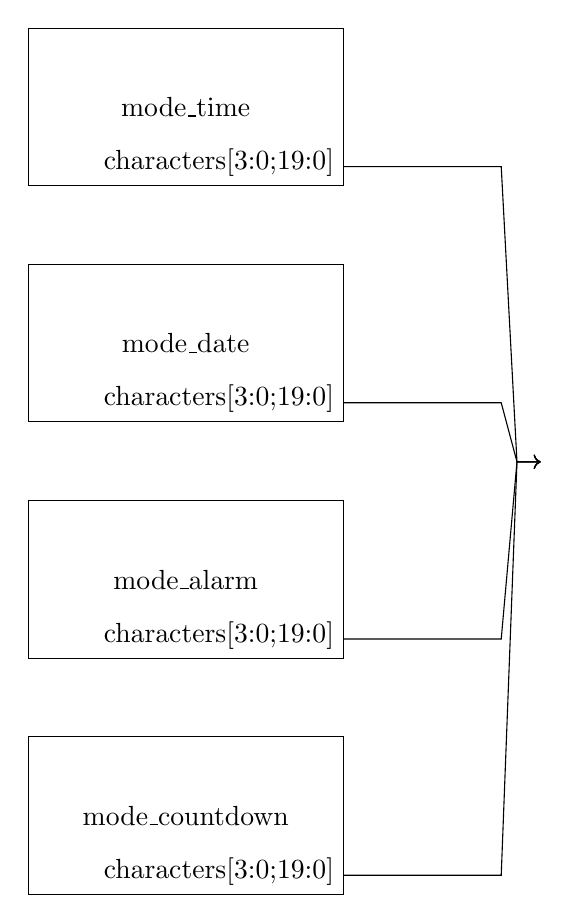
\begin{tikzpicture}
      \label{uhrenbaustein_char}
    %  \draw[help lines] (0, -10) grid (15, 2);

      \node [rectangle, draw=black, minimum height= 2cm, minimum width = 4cm, above left] at (4, -2) {mode\_time};
      \node [above left] at (4, -2) {characters[3:0;19:0]};

      \node [rectangle, draw=black, minimum height= 2cm, minimum width = 4cm, above left] at (4, -5) {mode\_date};
      \node [above left] at (4, -5) {characters[3:0;19:0]};

      \node [rectangle, draw=black, minimum height= 2cm, minimum width = 4cm, above left] at (4, -8) {mode\_alarm};
      \node [above left] at (4, -8) {characters[3:0;19:0]};

      \node [rectangle, draw=black, minimum height= 2cm, minimum width = 4cm, above left] at (4, -11) {mode\_countdown};
      \node [above left] at (4, -11) {characters[3:0;19:0]};



      \draw[->] (4, -1.75) --(6, -1.75) --(6.2, -5.5)->(6.5, -5.5);
      \draw[->] (4, -4.75) --(6, -4.75) --(6.2, -5.5)->(6.5, -5.5);
      \draw[->] (4, -7.75) --(6, -7.75) --(6.2, -5.5)->(6.5, -5.5);
      \draw[->] (4, -10.75)--(6, -10.75)--(6.2, -5.5)->(6.5, -5.5);




%      \draw[line width=2pt,->] (-1, -0.5) -> (0, -0.5) node[right] { enable\_gen };
%      \draw[line width=2pt,->] (-1, -1.5) -> (0, -1.5) node[right] { dcf77\_eval };
%      \draw[line width=2pt,->] (-1, -2.5) -> (0, -2.5) node[right] { key\_control };

%      \draw[->] (6,-0.5)node[left] {d\_en}   -- ++(2, 0);
%      \draw[->] (6,-1)  node[left] {d\_rw}   -- ++(2, 0);
%      \draw[->] (6,-1.5)node[left] {d\_rs}   -- ++(2, 0);
%      \draw[line width=2pt,->] (6,-2) node[left] {d\_data} -- ++(2, 0);
%
%      \draw[->] (6,-3)  node[left] {al\_on} -- ++(2, 0);
%      \draw[->] (6,-3.5)node[left] {su\_on} -- ++(2, 0);
%      \draw[->] (6,-4)  node[left] {ti\_on} -- ++(2, 0);
%      \draw[->] (6,-4.5)node[left] {ti\_beep} -- ++(2, 0);

%      \draw (0,0) rectangle (6, -5);
    \end{tikzpicture}
  \end{center}
  \caption{Block diagram of uhrenbaustein}
\end{figure}


\begin{figure}
  \begin{center}
    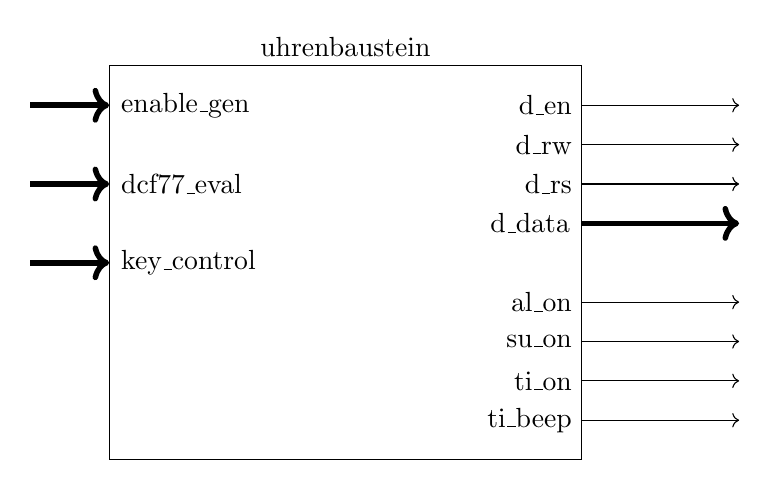
\begin{tikzpicture}
      \label{uhrenbaustein_time}
%      \draw[help lines] (-2, -8) grid (7, 2);

      \node[above] at (3,0) {uhrenbaustein};

      \draw[line width=2pt,->] (-1, -0.5) -> (0, -0.5) node[right] { enable\_gen };
      \draw[line width=2pt,->] (-1, -1.5) -> (0, -1.5) node[right] { dcf77\_eval };
      \draw[line width=2pt,->] (-1, -2.5) -> (0, -2.5) node[right] { key\_control };

      \draw[->] (6,-0.5)node[left] {d\_en}   -- ++(2, 0);
      \draw[->] (6,-1)  node[left] {d\_rw}   -- ++(2, 0);
      \draw[->] (6,-1.5)node[left] {d\_rs}   -- ++(2, 0);
      \draw[line width=2pt,->] (6,-2) node[left] {d\_data} -- ++(2, 0);

      \draw[->] (6,-3)  node[left] {al\_on} -- ++(2, 0);
      \draw[->] (6,-3.5)node[left] {su\_on} -- ++(2, 0);
      \draw[->] (6,-4)  node[left] {ti\_on} -- ++(2, 0);
      \draw[->] (6,-4.5)node[left] {ti\_beep} -- ++(2, 0);

      \draw (0,0) rectangle (6, -5);
    \end{tikzpicture}
  \end{center}
  \caption{Block diagram of uhrenbaustein}
\end{figure}




\end{document}
